\section{Zielsetzung}
\label{sec:Zielsetzung}

In dem Versuch He-Ne-Laser sollen die Grundlagen der Lasertechnik kennengelernt
werden. Diese wird zunächst anhand der theoretischen Grundlagen beleuchtet und
im Experiment durch einen Helium-Neon-Laser untersucht werden.

\section{Theorie}
\label{sec:Theorie}
% Vorschlag für den Beginn, damit nicht andauernd zitiert werden muss.
Die folgende theoretische Beschreibung von optischen Geräten wie Laser ist aus den Quellen
\cite{anleitung} und \cite{eichler} entnommen. Laser erzeugen einen möglichst monochromatischen
Lichtstrahl mit hoher Kohärenz, Intensität und Polarisation. Bei der theoretischen
Beschreibung der Funktionsweise sind Wechselwirkungen eines Strahlnfeldes mit einem
System aus Atomen zu analysieren. Eine theoretisches Modell hierfür bietet ein
Zweiniveausystem.

\subsection{Zweiniveausystem}
Ein einfaches Modell zur Beschreibung eines Systems aus Atomen ist das Zweiniveausystem.
Werden Zustände $\shortmid 1 \rangle$ und $\shortmid 2 \rangle$ mit entsprechenden
Eigenwerten $E_1$ und $E_2$ ($E_1<E_2$). Durch Absorption und Emission eines Photons mit
Energie $h\nu=E_2-E_1$ kann das System zwischen den Zuständen springen. Dabei sind
folgende Prozesse für die Lasertechnik wichtig:
\begin{itemize}
  \item induzierte Absorption:
  Hier wird durch Absorption eines Photons das System in Zustand $\shortmid 2 \rangle$
  gehoben. Die Wahrscheinlichkeit, mit der dieser Prozess stattfindet, wird beschrieben
  Durch
  \begin{equation}
    P_{1\rightarrow 2} = B_{1\tightarrow 2}\cdot \rho(\nu).
  \end{equation}
  Dabei stellt $P_{1\rightarrow 2}$ die Übergangswahrscheinlichkeit, $B_{1\rightarrow 2}$ den
  Einsteinkoeffizienten für die induzierte Absorption und $\rho(\nu)$ die spektrale Energiedichte
  eines externen Strahlungsfeldes da.
  \item induzierte Emission:
  Hierbei stimmt das induzierte Photon in Energie, Phase und Ausbreitungsrichtung
  mit dem anregenden Photon überein. Hier kann eine analoge Beschreibung wie bei der
  induzierten Emission verwendet werden. Somit wird die Übergangswahrscheinlichkeit durch
  \begin{equation}
    P_{2\rightarrow 1} = B_{2\rightarrow 1}\cdot\rho(\nu)
  \end{equation}
  definiert. $B_{2\rightarrow 1}$ stellt hier den Einsteinkoeffizienten der induzierten
  Emission da.
  \item spontane Emission:
  Auch unabhängig von einer externen Strahlnfeldes kann ein Photon emittiert werden
  Dabei gilt die Beziehung
  \begin{equation}
    P_s = A_{2\rightarrow 1}
  \end{equation}
  mit dem Einsteinkoeffizienten $A_{2\rightarrow 1}$.
\end{itemize}

Befindet sich ein System im thermischen Gleichgewicht, so kann es durch die
Besetzungszahlen $n_i$ der Niveaus beschrieben werden. Diese folgen der Boltzmann-Statistik
\begin{equation}
    n_i = \frac{g_in}{Z}\exp{-\frac{E_i}{k_\text{B}T}}
\end{equation}
Als $n$ wird die gesamtzahl der Systeme, $g_i$ das statistische Gewicht dess Zustandes
$\shortmid i \rangle$ und Zals die Zustandssumme bezeichnet. Durch den Einsatz
eines Lasers soll dafür gesorgt werden, das eine dauerhafte Verstärkung des
Strahlungsfeldes entsteht.

\subsection{Aufbau und Funktionsweise eines Lasers}
Ein Laser kurz für "Light Amplification by Stimulated Emission of Radiation" besteht prinzipiell aus
drei Teilen. Dem aktiven Lasermedium, einer Pumpquelle und einem Resonator. Dieser
schematische ist in Abbildung \ref{pic:laser} zu sehen.
\begin{figure}[htb]
  \centering
  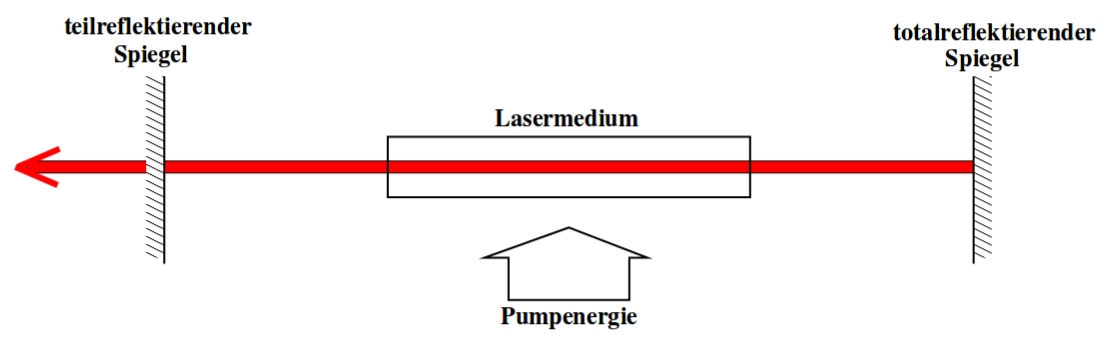
\includegraphics[width=0.8\textwidth]{content/prinzip_laser.png}
  \caption{Schematischer Aufbau eines Lasers mit Pumpquelle, aktivem Medium und Resonator.}
  \label{pic:laser}
\end{figure}
Um mindestens einen angereten Zustand mehr im aktiven zu haben wie Grundzustände,
wird eine Pumpquelle verwendet um diese Besetzungsinverssion herzustellen.
Daraufhin tritt in dem aktiven Medium mehr induzierte Emission als spontane auf und das
Strahlungsfeld wird verstärkt. Damit der Laufweg der Photonen möglichst groß wird, verlängert
der Resonator genau diesen durch zwei gegenüberliegende Spiegel. Einer dieser Spiegel
muss halbdurchlässig sein, um einen erzeugten Strahl auskoppeln zu können. Durch eine
konfokale Anordnung werden Verluste minimiert.
Ein langer Laufweg ist wichtig, da so ein Photon öfters durch das Lasermedium gelangen kann
und dadurch weitere Emissionen bewirkt.
Im Resonator können nur Wellenlängen verstärkt werden,welche die Bedingung
\begin{equation}
  \lambda = \frac{2L}{n}\ \ n\in\mathds{N}
\end{equation}
erfüllen. Hierbei ist $L$ der Abstand zwischen den Spiegeln und n der Index der Moden.
Durch diese Bedingung tritt eine Selektion der Wellelängen auf, die bedtrachtet werden können.
Innerhalb eines durch den optischen Dopplereffekt auftretenden natürlichen Spektrums
sind diese longitudinale Moden.

Treten stationäre Intenstiätsverteilungen durch Beugungseffekte an Unebenheiten
der Spiegel senkrecht zur Rotationachse auf, so werden diese als transversale oder
TEM-Moden ($transversal electromagnetic$) bezeichnet.

Wird die Intensität $I_{00}$ der Grund- oder Fundamentalmode $T_{00}$ betrachtet, so
folgt sie einer Gaußverteilung der Form
\begin{equation}
  I_{00} = I_0 \text{e}^{-2\left(\frac{d-d_0}{w}\right)^2}.
\end{equation}
$w$ wird als Radius der Fundamentalmode und $d$ als senkrechter Abstand zur Resonatorachse
bezeichnet. Die nächsthöhere Mode, die $T_{01}$-Mode wird beschrieben durch
\begin{equation}
  I_{01}(d) = I_{0,1}\text{e}^{-2\left(\frac{d-d_{0,1}}{w_1}\right)^2}+I_{0,2}\text{e}^{-2\left(\frac{d-d_{0,2}}{w}\right)^2}
\end{equation}
Es tritt hier eine heoretisch nicht erwartete Asymmetrie in der Hohe der beiden Maxima,
d.h. $I_{0,1} \neq I_{0,2}$ auf.
Stabile Moden treten auf, wenn die Stabilitätsbedingung
\begin{equation}
  0\leq g_1g_2\leq 1
\end{equation}
auftritt. Dabei beschreibt
\begin{equation}
  g_i = 1 - \frac{L}{r_i}
\end{equation}
mit dem Krümmungsradius $r_i$. In Abbildung \ref{fig:stabilität} ist das Produkt $g_1g_2$
als Funktion des Spiegelastandes $L$  für $r_2 = \SI{1400}{\metre}$ dargestellt. Wird ein
ebener Spiegel ("$r_1 = \infty$") betrachtet, so ergibt sich eine Bedingung für
$L$ von
\begin{equation}
  \SI{0}{\metre} \leq L \leq \SI{1.4}{\metre}.
\end{equation}
Ein Spiegel mit $r_1 = \SI{1400}{\milli\metre}$ ergibt
\begin{equation}
    \SI{0}{\metre} \leq \L \leq \SI{2.8}{\metre}.
\end{equation}

\begin{figure}
  \centering
  \includegraphics[width=0.8\textwidth]{build/stabilitaet.pdf}
  \caption{Darstellung der Stabilitätsparameter in Abhängigkeit der
  Resonatorlänge $L$.}
  \label{fig:Stabilität}
\end{figure}

\subsection{Helium-Neon-Laser}
\label{sec:Helium-Neon-Laser}
Bei einem Helium-Neon-Laser (HeNe-Laser), wie er in diesem Versuch verwendet wird,
besteht das Resonatormedium aus fünf Teilen Neon und einem Teil Helium, welches
bei einem Druck von $\SI{1}{\milli\bar}$ in einem Glaskolben eingeschlossen wird.
Durch Gasentladung wir ein Heliumkern in die $2^1s$ und $2^3s$ Zustände angeregt,
welches durch Stöße zweiter Art die $5s$ und $4s$ Zustände der Neonatome anregt.
Dies ist in Abbildung \ref{fig:HeNe} dargestellt.
\begin{figure}
  \centering
  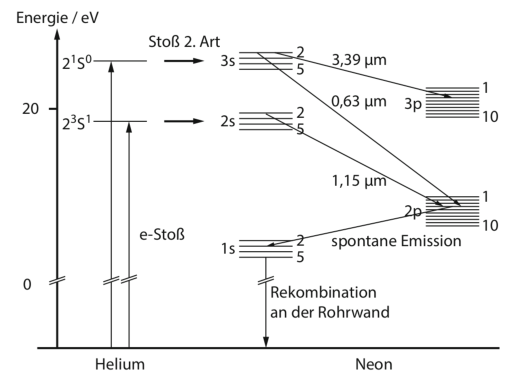
\includegraphics[width=0.8\textwidth]{content/HeNe.pdf}
  \caption{Schematische Darstellung der Übergänge zur stimulierten
  Emission eines HeNe-Lasers \cite[68]{eichler}.}
  \label{fig:HeNe}
\end{figure}

Da der $5s$ Zustand des Heliums eine größere mittlere Lebensdauer hat als der $3s$ Zustand,
ist die Besetzungsinversion erfüllt und wahrscheinlicher als spontane Emissionen.
Die bei diesem Übergang auftretende Spektrallinie zwischen den beiden Neonatomen liegt bei
$lambda = \SI{632.8}{\nano\metre}$ und damit im sichtbaren roten Bereich des elektromagnetischen
Spektrums.

% \begin{equation}
% Für Formeln
%   \label{eqn:Formel}
% \end{equation}
